\documentclass[journal]{IEEEtran}
\usepackage{graphicx}
\usepackage{amsmath}
\usepackage{subcaption}
\usepackage{mwe}
\begin{document}

\title{Autonomous RF Trigger Threshold Control and Systems Integration for the ARIANNA HRA-7}

\author{John-Paul Gomez-Reed and Jordan C. Hanson, \textit{Whittier College Dept. of Physics and Astronomy}
\thanks{Special thanks to Prof. F. Radoniqi, Whittier College Dept. of Business Administration, and the Ondrasik-Groce Fellowship.}}

\markboth{IEEE Transactions on Nuclear Science,~Vol~xx,~No.xx}
{G\'{o}mez-Reed and Hanson: Autonomous RF Trigger Threshold Control and Systems Integration for the ARIANNA HRA-7}

\maketitle

\begin{abstract}
We report on the development of an autonomous control system for radio-frequency (RF) detectors as part of the Antarctic Ross Ice-shelf Antenna Neutrino Array (ARIANNA) project.  The ARIANNA science goal is to observe ultrahigh energy (UHE, $>10^{17}$ eV) cosmogenic neutrinos using an autonomous array of RF detectors on the Ross Ice Shelf.  UHE neutrinos (UHE-$\nu$) undergo the Askaryan effect in ice, producing RF pulses (100-500 MHz).  The systems consist of RF detection channels and continuously-running digital acquisition circuits named SSTs.  \textit{Trigger logic} requires signals in multiple channels to exceed SST voltage thresholds before the SSTs are stopped.  Once the SSTs are stopped the RF data is saved by software running on an ARM microcontroller called the MBED. Thermal noise from the RF channel amplifiers randomly exceeds thresholds at a rate proportional to the SST sampling rate, and the thermal noise rate is a steeply falling function of threshold voltage.  The dependence is so sensitive that even in RF-quiet areas of Antarctica, thresholds must be fine-tuned to optimize sensitivity to low signal-to-noise ratio (SNR) pulses, while avoiding thermal rate fluctuations of several orders of magnitude.  We solve the problem by introducing FPGA firmware and MBED software to empower detectors to tune thresholds \textit{autonomously}.  A multi-mode frequency counter (MMFC) measures the thermal rate from the SSTs and saves the data in block RAM.  The trigger rate is measured correctly ($<1\%$ error) by the MMFC in the range (1 Hz - 1 MHz) in lab-bench and on-board scenarios.  Further, the trigger rate of thermal noise from the RF chain, as a function of voltage threshold, is measured correctly by the MMFC and shown to follow theoretical expectations.  Rate measurements are transmitted via SPI protocol from firmware to the MBED.  An updated threshold value is passed from the MBED via SPI to an on-board DAC controlling the SST threshold.  A system feedback loop is established between the SST, the FPGA, and the MBED, to optimize SST thresholds.  The solution replaces time-consuming manual threshold adjustment, allowing the expansion of the ARIANNA array to hundreds of stations.
\end{abstract}
\IEEEpeerreviewmaketitle

\section{Introduction}

\IEEEPARstart{O}{ver} 100 years after the discovery of UHE cosmic rays (UHECRs), their origin remains a mystery. Representing the highest-energy sub-atomic particles observed in nature, UHECRs could provide a wealth of information about high-energy astrophysics and particle physics if detected and traced to their sources.  However, the deflection of charged UHECRs by magnetic fields in the cosmos impedes the identification of their origin.  UHE neutrinos, however, traverse the cosmos unimpeded and point back to their origin.  UHE neutrinos are linked to UHECR production in two ways.  The first type, called \textit{astrophysical} neutrinos, are produced at sources via the acceleration of charged cosmic rays and the subsequent UHECR interactions with gas surrounding the source.  The second type, called \textit{cosmogenic} neutrinos, are born from the decay of UHECRs while propagating through the universe via interactions with photons from the cosmic microwave background (CMB).  The latter process is called the GZK effect.  Recently, the IceCube detector at the South Pole reported a UHE neutrino detection with reconstructed energy $\approx 3 \times 10^{14}$ eV, from the same celestial coordinates as a flaring $\gamma$-ray blazar.  If the same physics driving the $\gamma$-ray emission created the UHE neutrino, it would imply UHECR production from a known high-energy astrophysical source.

Although cosmic-ray sources of lower energies have been identified (cite, cite), UHE neutrinos represent a promising pathway to identifying the UHECR sources.  To detect UHE-$\nu$ signals, detection instrumentation must be deployed through kilometer-scale volumes of dense matter due to the low interaction probability of UHE-$\nu$.  In the past decade, the astroparticle physics community has targeted ice formations in Antarctica and Greenland as detection media.  These locations are ideal because optical and RF signals created by UHE-$\nu$ interactions propagate efficiently through ice.  Further, the ice sheets and ice shelves of Antarctica typically have low man-made RF interference and are so large that massive detectors can be designed.  The IceCube detector observes optical Cherenkov photons generated by UHE-$\nu$ in a 1 km$^3$ volume of ice beneath the South Pole (cite).  Optical photons travel $l = \mathcal{O}(100)$ m in the ice (cite).  However, UHE-$\nu$ are also expected to produce RF-emissions via the Askaryan effect (cite).  In the case of RF radiation, the relevant propagation distance increases: $l = \mathcal{O}(1)$ km (cite, cite).  By constructing an array of relatively inexpensive RF pulse detectors spaced by $l$ in ice, overall designs achieving greater than $10^{12}$ metric tonnes of ice are within reach.  Such enormous fiducial volumes would provide a medium large enough to detect UHE-$\nu$ fluxes from across the cosmos (cite).

\IEEEPARstart{T}{he} ARIANNA project is an array of autonomous UHE neutrino detectors stations that are used to detect and record ultra high energy neutrinos, and other cosmic rays, using RF.  Although there are many iterations of the ARIANNA station deployed in Antarctica, they all share hardware that allows them to process RF signals via analog RF signals.  This is done through 4 or 8 SMA channels that are processed by both an  Synchronous Sampling and Trigger (SST) I.C. and an FPGA.  The SST verifies if a signal crosses both a low and high voltage threshold, where it then sends that signal to the Spartan-3 FPGA to determine if the proper number of channels, 1 to 4, were triggered.  If both conditions are satisfied, the FPGA then begins to record the signal via FPGA RAM, where it is held until the MBED microcontroller initiates an SPI communication protocol and then records this data onto an SD card.  During this process, the voltage thresholds serve as a means to filter incoming signals and prevent false positives from being recorded on the ARIANNA board's limited memory resources.  At the present, these voltage thresholds are an imperfect solution as they must be manually set on each ARIANNA station, leading to issues of potential data loss, wasted memory resources, and project scope limitation.  Due to the harsh nature of the environment, the weather could prevent an individual from setting the voltage threshold, which can lead to one of two conditions: voltage thresholds being too high or too low.  If the magnitude of the voltage thresholds are too low, false positives will be recorded, leading to wasted memory resources; conversely, having voltage thresholds that are too high will lead to potential data loss as true positives will not be recorded.  Furthermore, increasing the number of deployed ARIANNA stations is infeasible as it would require a person or a team to manually set a large number of stations by hand.

Our group has been developing the firmware and software further so that the ARIANNA station can automate the process of adjusting its own voltage thresholds.  A new component, dubbed the Multi-mode Frequency Counter (MMFC), has been successfully integrated into the ARIANNA firmware and software with the intention that it will serve as a means to monitor the individual high and low lines of the ARIANNA motherboard so that it may better react to changes in both the long and short term.  The MMFC is able to measure frequencies from 20 Hz to 25 MHz within a 10 \% error range, but given proper adjustments and testing, it can potentially measure lower frequencies and up to 80 MHz.  

\begin{figure*}[h!]
	\centering
	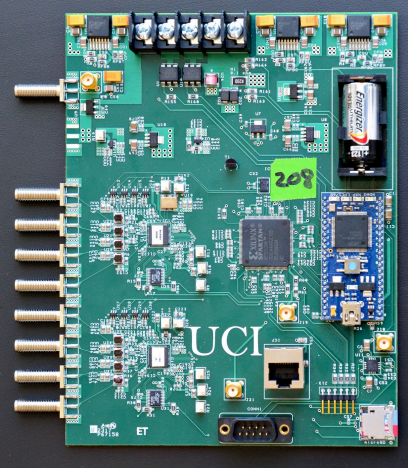
\includegraphics[scale=0.55]{mboard.png}
	\caption{An 8-channel ARIANNA motherboard.}
	\label{ARIANNA motherboard}
\end{figure*}


% You must have at least 2 lines in the paragraph with the drop letter
% (should never be an issue)

%\hfill mds
 
%\hfill August 26, 2015

%\subsection{Subsection Heading Here}
%Subsection text here.

% needed in second column of first page if using \IEEEpubid
%\IEEEpubidadjcol

%\subsubsection{Subsubsection Heading Here}
%Subsubsection text here.


% An example of a floating figure using the graphicx package.
% Note that \label must occur AFTER (or within) \caption.
% For figures, \caption should occur after the \includegraphics.
% Note that IEEEtran v1.7 and later has special internal code that
% is designed to preserve the operation of \label within \caption
% even when the captionsoff option is in effect. However, because
% of issues like this, it may be the safest practice to put all your
% \label just after \caption rather than within \caption{}.
%
% Reminder: the "draftcls" or "draftclsnofoot", not "draft", class
% option should be used if it is desired that the figures are to be
% displayed while in draft mode.
%
%\begin{figure}[!t]
%\centering
%\includegraphics[width=2.5in]{myfigure}
% where an .eps filename suffix will be assumed under latex, 
% and a .pdf suffix will be assumed for pdflatex; or what has been declared
% via \DeclareGraphicsExtensions.
%\caption{Simulation results for the network.}
%\label{fig_sim}
%\end{figure}

% Note that the IEEE typically puts floats only at the top, even when this
% results in a large percentage of a column being occupied by floats.


% An example of a double column floating figure using two subfigures.
% (The subfig.sty package must be loaded for this to work.)
% The subfigure \label commands are set within each subfloat command,
% and the \label for the overall figure must come after \caption.
% \hfil is used as a separator to get equal spacing.
% Watch out that the combined width of all the subfigures on a 
% line do not exceed the text width or a line break will occur.
%
%\begin{figure*}[!t]
%\centering
%\subfloat[Case I]{\includegraphics[width=2.5in]{box}%
%\label{fig_first_case}}
%\hfil
%\subfloat[Case II]{\includegraphics[width=2.5in]{box}%
%\label{fig_second_case}}
%\caption{Simulation results for the network.}
%\label{fig_sim}
%\end{figure*}
%
% Note that often IEEE papers with subfigures do not employ subfigure
% captions (using the optional argument to \subfloat[]), but instead will
% reference/describe all of them (a), (b), etc., within the main caption.
% Be aware that for subfig.sty to generate the (a), (b), etc., subfigure
% labels, the optional argument to \subfloat must be present. If a
% subcaption is not desired, just leave its contents blank,
% e.g., \subfloat[].


% An example of a floating table. Note that, for IEEE style tables, the
% \caption command should come BEFORE the table and, given that table
% captions serve much like titles, are usually capitalized except for words
% such as a, an, and, as, at, but, by, for, in, nor, of, on, or, the, to
% and up, which are usually not capitalized unless they are the first or
% last word of the caption. Table text will default to \footnotesize as
% the IEEE normally uses this smaller font for tables.
% The \label must come after \caption as always.
%
%\begin{table}[!t]
%% increase table row spacing, adjust to taste
%\renewcommand{\arraystretch}{1.3}
% if using array.sty, it might be a good idea to tweak the value of
% \extrarowheight as needed to properly center the text within the cells
%\caption{An Example of a Table}
%\label{table_example}
%\centering
%% Some packages, such as MDW tools, offer better commands for making tables
%% than the plain LaTeX2e tabular which is used here.
%\begin{tabular}{|c||c|}
%\hline
%One & Two\\
%\hline
%Three & Four\\
%\hline
%\end{tabular}
%\end{table}


% Note that the IEEE does not put floats in the very first column
% - or typically anywhere on the first page for that matter. Also,
% in-text middle ("here") positioning is typically not used, but it
% is allowed and encouraged for Computer Society conferences (but
% not Computer Society journals). Most IEEE journals/conferences use
% top floats exclusively. 
% Note that, LaTeX2e, unlike IEEE journals/conferences, places
% footnotes above bottom floats. This can be corrected via the
% \fnbelowfloat command of the stfloats package.




\section{Methods}
\subsection{Specification/Operation:}
The MMFC was designed to calculate frequencies within a range of 6 orders of magnitude, where the minimum and maximum of this range can be adjusted by changing the comparison/simulated clock frequency within the FPGA program; it should be noted that the maximum of this 6 order magnitude range cannot exceed 80 MHz as this is the maximum value that the MMFC can detect as it runs on 160 MHz clock.  A general assumption is that signals that enter the ARIANNA board will be of a lower frequency than 80 MHz, so the input signal being measured by the MMFC is triple registered.  Triple registering a signal is a process which involves an input signal's value being cascaded through three registers so that the signal's value is not metastable and so that the MMFC can detect a signal's falling edge (signal value goes from 1 to 0); if a falling edge is detected, a 16-bit register (signal counter) is incremented.  At the same time, another 16-bit register is being incremented by a comparison/simulated clock (clock counter), which is the running clock frequency divided by a constant.  When one of these two registers are filled, both stop incrementing and the FPGA holds each value until it receives the proper signal to transfer the data from MMFC to register based FIFOs so that the data can be ready for the MBED mircrocontroller's signal to initiate an SPI communication protocol.  After the FPGA has communicated with the MBED microcontroller, the 16-bit registers will reset and then FPGA will repeat these operations until the power is shut off.  
%Subsection text here.
\subsection{Theory:}
Once the MMFC reports both counters, the microcontroller will then input the values found into this equation: 
\begin{equation*}
f_s = \left(\frac{c_s}{c_c}\right)*f_c
\end{equation*}
Where $f_s$ is the frequency of the signal, $c_s$ is the number of rising edges from the input signal encountered, $c_c$ is the number of counts that the clock counter made, and $f_c$ is the frequency of the comparison/simulated clock. 

\begin{figure*}
	\centering
	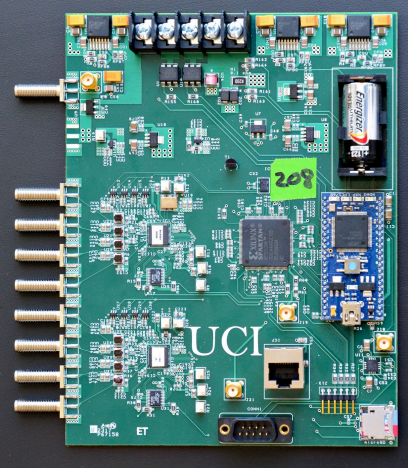
\includegraphics[scale=0.08]{mboard.png}
	\caption{Test 1, where the ARIANNA board is connected to AFG line of the MDO3024.}
	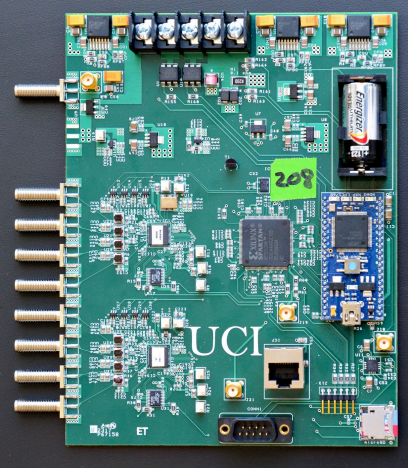
\includegraphics[scale=0.08]{mboard.png}
	\caption{Test 2, where the ARIANNA board is connected to an amplifier.}

\end{figure*}

\subsection{Experimental Setup:}
The experiment was set up as seen in the figure.  An MDO3024  served as an Arbitrary Function Generator (AFG) and as a means to send a measurable signal into the ARIANNA board.  The AFG had a frequency range of 500 mHz to 25 MHz and as such limited measurements to this range.  The AFG was connected to the ARIANNA board via a BNC female to BNC female cable and BNC to SMA female connector.  A USB-Mini cord was then attached to the microcontroller so that the microcontroller can communicate with the PC via a terminal program (PuTTY).  To power the board a DC regulated power supply was used and set to 12.2 V.  The ARIANNA board was also connected to a Platform Cable USB II, which allowed the FPGA to be reprogrammed.  During these tests, voltage thresholds were set to 1228 counts on the low end and 1750 on the high end and so the AFG positive and negative thresholds were adjusted to reach above and below these thresholds (902 mV and -650 mV).  

The MMFC was then tested using a 3.3 V frequency amplifier.  Similarly to the previous test, the amplifier was plugged into the ARIANNA motherboard via a male BNC to female SMA on the input of the ARIANNA board to a male BNC to female SMA on the output of the amplifier, while the amplifier’s input has a $50\Omega$ terminator attached.  The amp’s power source was then connected to the ARIANNA board using another female SMA to male BNC connector using a test clip.  

The MMFC in conjunction with the ARIANNA’s trigger settings were then tested using a similar setup to the first tests but the changes were within the software rather than the hardware.
\subsection{Procedure:}
The MMFC was designed to only listen to one signal at a time, so two tests were conducted on each channel when changing between the low and high lines of a single channel.  When changing between lines or channels, the board was reset by removing power from the board in its entirety and disconnecting the MBED microcontroller from the PC; when changing SMA channels the AFG is shut down as well.  Once prep is complete, the AFG is turned on and set to a frequency in the Hz range and then increased from there.  The value that the FPGA reads is then output to the terminal and once a certain number of tests are conducted at one frequency, the frequency is increased until 25 MHz is reached; this process was then repeated for each of the four channels. 
	 
In the second test, the procedure is that the voltage thresholds of the ARIANNA board are modified.  In between tests, the SD card on the ARIANNA board was removed and reprogrammed on a PC and then the ARIANNA system was restarted to begin recording data.  There were only two tests completed, a single test on both the high and low lines of a single channel; when testing a line, only the threshold associated with that line was changed, while the other was kept at the original value.  

The trigger settings were tested using one channel, channel 0 or the first of the four channels, in order to test the results of the four combinations of the trigger settings: individual settings turned on, both settings on, and both settings off, although it should be noted that dual threshold triggering was tested on the previous tests conducted, so the other three combinations were more of the focus of these sets of tests.  The same tests were conducted as the previous experiment entailed.


\begin{figure*}[!htb]
	
	\begin{subfigure}[t]{0.5\linewidth}
		\centering
		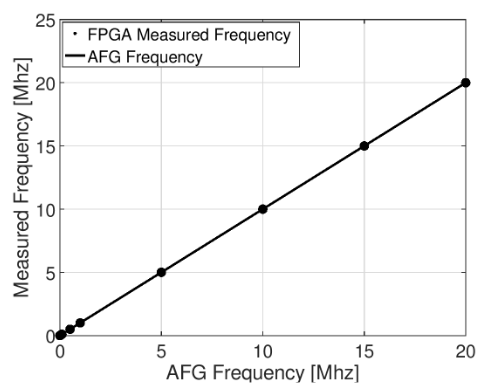
\includegraphics[scale=0.4]{fpgaff.png}
		\caption{MMFC frequency measurement performance within a Spartan-6 test board.}
	\end{subfigure}
	\hfill
	\begin{subfigure}[t]{0.5\linewidth}
		\centering
		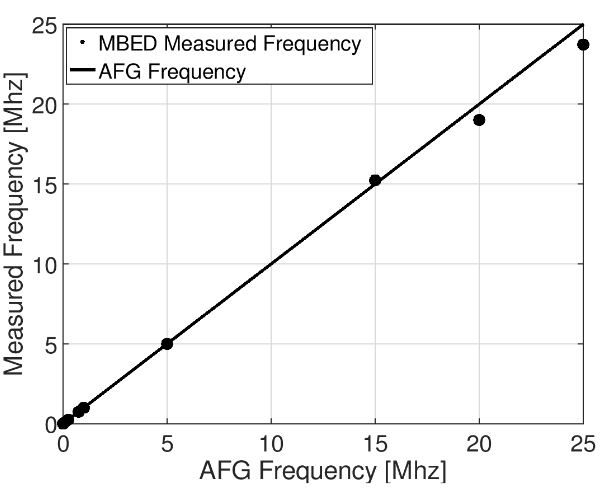
\includegraphics[scale=0.4]{mbedff.png}
		\caption{MMFC frequency measurement performance within the ARIANNA firmware and software.}
	\end{subfigure}

	\begin{subfigure}[b]{\linewidth}
	\centering
	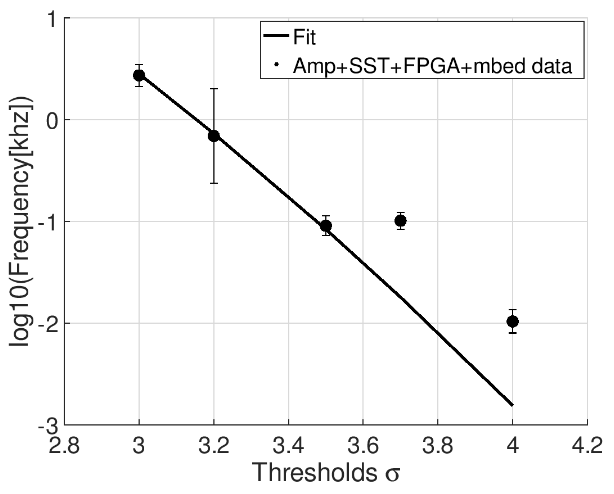
\includegraphics[scale=0.5]{scan.png}
	\caption{MMFC threshold measurement performance.}
\end{subfigure}

	\caption{MMFC performance tests.}
\end{figure*}

\section{Results}
	During both of the tests, the signal that was detected by the SST chip and measured by the MMFC were reported every minute when the system received a forced trigger (a non-environmental trigger) from the microcontroller and the data was output to the terminal on the PC that the microcontroller was connected to.  The program within the microcontroller made post-calculation adjustments to the data that was reported by shifting the data two bits to the left.  During the first test, the AFG was allowed to run on one frequency for about 3-4 minutes, about three measurements, where it was changed to another higher frequency starting from 10 Hz and rising to 25 MHz; each set of AFG measurements were then averaged.  Figure 4-a shows the results of the first test where the X-axis is the AFG output frequency, while the Y-axis is the MMFC measured frequency; there is also a line added to show the true behavior of the AFG.  During the second test, the ARIANNA motherboard and the amplifier were left to run for 1-3 hours on each set of $\sigma$ separated thresholds.  The data from these tests were then cleaned of rare high, low and null values, where they were then averaged and plotted.  Figure 4-c shows the results of the second test where the X-axis shows $\sigma$ threshold and the Y-axis shows the log10 measured frequency in kHz.  Figure 4-c also has a line representing the model used in order to determine the actual frequency that should be measured at a given threshold.

\section{Discussion}
	For the first test, it can be observed that at lower frequencies, measurements have some higher error and begins to stabilize as rates increase and then begin display the same behavior at higher rates for all four channels, similar to earlier experiments on previous experiments conducted on a Spartan-6 FPGA evaluation board.  In that experiment, as well as this one, it is shown that as the MMFC begins to record lower frequencies, the number of signal counts that can be detected by MMFC is incredibly limited and if the MMFC “misses” a single count.  As for larger frequencies, it was found that the MDO3024 begins to have trouble creating clean square wave signal. 	For the second test, it can be observed that at lower $\sigma$ thresholds, the measured frequencies match or are close to the model, while at higher thresholds there is greater deviation.  Also, in the "3.2 $\sigma$ threshold" test, the error bar is much higher than the other measurements.  Both errors are still being explored, although there are some theories as to why the first error in the second test occurs.  A theory for the model not being matched may be fluctuations in setting the voltage thresholds; when initially setting the value of the voltage threshold may actually shift, so it could be above or below the intended value.  The second error is not explainable because during the test run, null values were measured and this error never occurred in lower or higher threshold values.  An error that was contained in all tests was a rightward circular shift of two bits, which caused an error of ±3 counts to be present within each data reading.  While a small number, it begins to matter when dealing with smaller frequencies in the Hertz frequency range as a missed count can lead to an answer with an incredibly high error.  This may be due to many sources, some may be, the component holding the data, the data streaming, and/or the way the data is moved on the FPGA.  In the standard ARIANNA FPGA architecture, there are no register based FIFOs, so this could be a source of error.

\section{Conclusion}
The deployed ARIANNA stations suffer from the thermal noise and other man-made activities as it affects their ability to record data effectively, in response to this, manually set voltage thresholds are used to filter out incoming signals so that false-positives are not recorded.  This is an imperfect solution as false positives can still be recorded if the magnitudes of the voltage thresholds are not set correctly or on time; in this study, an FPGA component, the MMFC, was implemented in an attempt to automate this process so that ARIANNA stations can react to any major changes in the environment.  The MMFC was integrated into the ARIANNA firmware and software and it was tested using an AFG and a frequency amplifier; the AFG was used to see if the MMFC could measure input signals correctly, while the amplifier was used to see if it could measure the correct frequency when given different thresholds.  The AFG test showed that despite being integrated into the ARIANNA firmware, the MMFC could still measure input frequencies with good accuracy, although it began to deviate from it when reaching into higher frequencies.  The amplifier test showed that at lower $\sigma$ thresholds, the MMFC fits the model, while at higher $\sigma$ thresholds the MMFC deviates from the model greatly.  The errors in the first test could be explained by the fact that at lower frequencies, the MMFC misses a count and causes the error to spike, while at higher frequencies, the MDO3024 is to blame as the AFG is reaching the end of its bandwidth.  The errors in the second test could be explained by the fact that there may be fluctuations in the value of the voltage thresholds, so the actual value may be higher or lower than the intended value.  The errors revealed in both tests could be from the fact that in order to integrate the MMFC, register based FIFOs were used to allow the data from the MMFC to be transported from the FPGA to the MBED microcontroller.  In general, this study was a means to see the feasibility of the integration of the MMFC into the ARIANNA motherboard and the results shows that more work is needed.  The main issue that needs to be solved is the deviation of the $\sigma$ threshold as this is the main crux of this study, if the MMFC cannot measure the correct frequency at a given threshold, then it will be unable to properly modify the voltage thresholds.  An improvement to these tests would be to add another MMFC; as it stands only one MMFC is operating and it only operates on the high line of the ARIANNA input signal logic, adding one to the low signal line and receiving the results could allow for the average value of an input frequency to be attained.  
% if have a single appendix:
%\appendix[Proof of the Zonklar Equations]
% or
%\appendix  % for no appendix heading
% do not use \section anymore after \appendix, only \section*
% is possibly needed

% use appendices with more than one appendix
% then use \section to start each appendix
% you must declare a \section before using any
% \subsection or using \label (\appendices by itself
% starts a section numbered zero.)
%



% you can choose not to have a title for an appendix
% if you want by leaving the argument blank


% use section* for acknowledgment
\section*{Acknowledgment}


The authors would like to thank the Ondrasik-Groce Fellowship, Whittier College, and Fatos Radoniqi for providing this research opportunity.


% Can use something like this to put references on a page
% by themselves when using endfloat and the captionsoff option.
\ifCLASSOPTIONcaptionsoff
  \newpage
\fi



% trigger a \newpage just before the given reference
% number - used to balance the columns on the last page
% adjust value as needed - may need to be readjusted if
% the document is modified later
%\IEEEtriggeratref{8}
% The "triggered" command can be changed if desired:
%\IEEEtriggercmd{\enlargethispage{-5in}}

% references section

% can use a bibliography generated by BibTeX as a .bbl file
% BibTeX documentation can be easily obtained at:
% http://mirror.ctan.org/biblio/bibtex/contrib/doc/
% The IEEEtran BibTeX style support page is at:
% http://www.michaelshell.org/tex/ieeetran/bibtex/
%\bibliographystyle{IEEEtran}
% argument is your BibTeX string definitions and bibliography database(s)
%\bibliography{IEEEabrv,../bib/paper}
%
% <OR> manually copy in the resultant .bbl file
% set second argument of \begin to the number of references
% (used to reserve space for the reference number labels box)
\begin{thebibliography}{1}

%\bibitem{IEEEhowto:kopka}
%H.~Kopka and P.~W. Daly, \emph{A Guide to \LaTeX}, 3rd~ed.\hskip 1em plus
%  0.5em minus 0.4em\relax Harlow, England: Addison-Wesley, 1999.
\bibitem{DesandInitPerfHRA3:barwick}
S.W.~Barwick, \emph{et al.} \emph{Design and Initial Performance of the HRA-3 Neutrino Detector Systems}. IEEE Transactions on Nuclear Science (2015).

\bibitem{Radarabs:Hanson}
J.C. Hanson, \emph{et al.} \emph{Radar absorption, basal reflection, thickness and polarization measurements from the Ross Ice Shelf, Antarctica}. Journal of Glaciology (2015).

\bibitem{Cosmog:Barwick}
S.W. Barwick, \emph{et al.} \emph{A first search for cosmogenic neutrinos with the ARIANNA Hexagonal Radio Array}. Astroparticle Physics Journal (2015)

\bibitem{Meta:Stephenson}
J Stephenson, \emph{et al.} \emph{Understanding Metastability in FPGAs [White Paper]}. Retrieved November 14, 2018 from Intel: https://www.intel.com/content/dam/www/programmable/us/en/pdfs/literature/wp/wp-01082-quartus-ii-metastability.pdf

\bibitem{SST:Kleinfelder}
S.A. Kleinfelder, \emph{et al.} \emph{The SST Multi-G-Sample/s Switched Capacitor Array Waveform Recorder with Flexible Trigger and Picosecond-Level Timing Accuracy} from:
arXiv:
https://arxiv.org/abs/1508.02460

\end{thebibliography}

% biography section
% 
% If you have an EPS/PDF photo (graphicx package needed) extra braces are
% needed around the contents of the optional argument to biography to prevent
% the LaTeX parser from getting confused when it sees the complicated
% \includegraphics command within an optional argument. (You could create
% your own custom macro containing the \includegraphics command to make things
% simpler here.)
%\begin{IEEEbiography}[{\includegraphics[width=1in,height=1.25in,clip,keepaspectratio]{mshell}}]{Michael Shell}
% or if you just want to reserve a space for a photo:

%\begin{IEEEbiography}{Michael Shell}
%Biography text here.
%\end{IEEEbiography}

% if you will not have a photo at all:
%\begin{IEEEbiographynophoto}{John Doe}
%Biography text here.
%\end{IEEEbiographynophoto}

% insert where needed to balance the two columns on the last page with
% biographies
%\newpage

%\begin{IEEEbiographynophoto}{Jane Doe}
%Biography text here.
%\end{IEEEbiographynophoto}

% You can push biographies down or up by placing
% a \vfill before or after them. The appropriate
% use of \vfill depends on what kind of text is
% on the last page and whether or not the columns
% are being equalized.

%\vfill

% Can be used to pull up biographies so that the bottom of the last one
% is flush with the other column.
%\enlargethispage{-5in}



% that's all folks
\end{document}


